\documentclass[10pt]{article}
\usepackage[ngerman]{babel}
\usepackage[utf8]{inputenc}
\usepackage[T1]{fontenc}
\usepackage{graphicx}
\usepackage[export]{adjustbox}
\graphicspath{ {./images/} }
\usepackage{amsmath}
\usepackage{amsfonts}
\usepackage{amssymb}
\usepackage[version=4]{mhchem}
\usepackage{stmaryrd}

\begin{document}
\section*{CT1 - Übungsaufgaben Einführung in Computertechnik}
Lösung

\begin{enumerate}
  \item Was ist Computertechnik? Formulieren Sie den Begriff mit eigenen Worten.\\
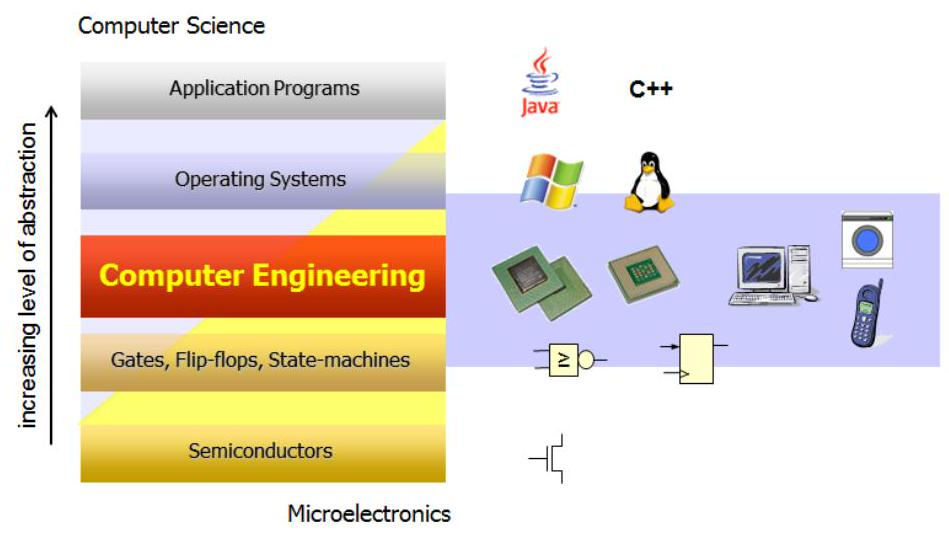
\includegraphics[width=\linewidth]{images/2025_01_02_f240dc33b50f25226887g-1(1)}
  \item Skizzieren Sie die Struktur eines Computersystems.\\
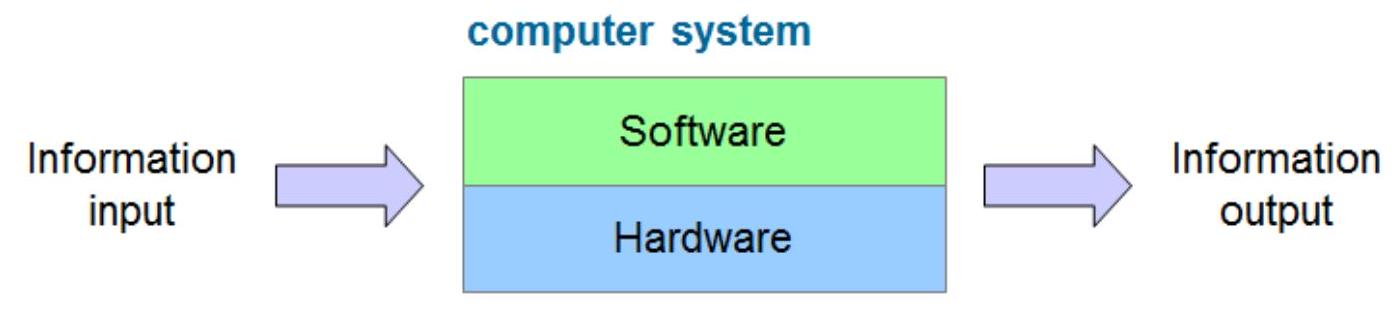
\includegraphics[width=\linewidth]{images/2025_01_02_f240dc33b50f25226887g-1}
  \item Nennen Sie die 4 grundlegenden Komponenten eines Rechnersystems und erklären Sie die Aufgabe jeder Komponente.
\end{enumerate}

\begin{center}
\begin{tabular}{|l|l|}
\hline
Name & Aufgabe \\
\hline
CPU & Central Processing Unit oder Prozessor \\
\hline
Memory & Instruktionen und Daten speichern \\
\hline
I/O &  \\
\hline
System-Bus & Elektrische Verbindung von Funktioneinheiten / Ausgabe Interface zu externen Devices \\
\hline
\end{tabular}
\end{center}

\section*{4. Erklären Sie die Aufgaben der Steuereinheit einer CPU.}
Die Steuereinheit liest, interpretiert und führt Instruktionen aus.\\
5. Erklären Sie die von Neumann Computer Architektur

\begin{itemize}
  \item instructions and data are stored in the same memory
  \item datapath executes arithmetic and logic operations and holds intermediate results
  \item control unit reads and interprets instructions and controls their execution\\
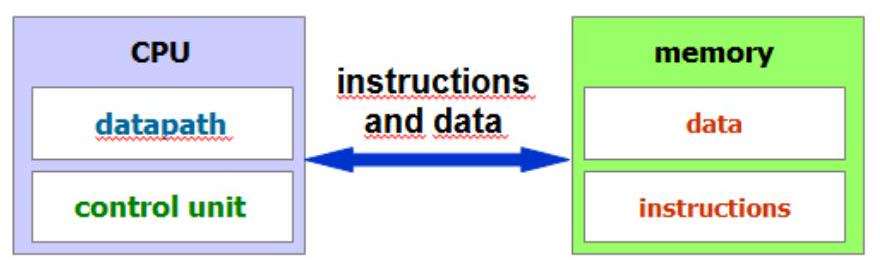
\includegraphics[width=\linewidth]{images/2025_01_02_f240dc33b50f25226887g-2}
\end{itemize}

\begin{enumerate}
  \setcounter{enumi}{5}
  \item Nennen und erklären Sie die 4 Schritte der Programmübersetzung. Welche Output Dateien werden erzeugt?
\end{enumerate}

\begin{center}
\begin{tabular}{|l|l|l|}
\hline
\begin{tabular}{l}
Name des \\
Schrittes (Tools) \\
\end{tabular} & Was macht der Schritt? & Output Datei \\
\hline
Preprocessor & \begin{tabular}{l}
Verarbeitet die Preprocessor Statements \\
(z.B. \#define, \#include) \\
Textprocessing: Ersetzen und Ergänzen \\
von Inhalten \\
\end{tabular} & \begin{tabular}{l}
Textfile mit modifiziertem \\
C Sourcecode \\
\end{tabular} \\
\hline
Compiler & \begin{tabular}{l}
Übersetzt C Sourcecode in \\
prozessorspezifische, symbolische \\
Assemblerbefehle. \\
\end{tabular} & \begin{tabular}{l}
Textfile mit \\
menschenlesbarem \\
Assemblercode \\
\end{tabular} \\
\hline
Assembler & \begin{tabular}{l}
Übersetzt Assemblercode in binäre \\
Maschinenbefehle \\
\end{tabular} & \begin{tabular}{l}
binäres Objectfile mit \\
Maschinenbefehlen \\
\end{tabular} \\
\hline
Linker & \begin{tabular}{l}
Fügt mehrere Objectfiles zu einem \\
ausführbaren Objektfile zusammen, löst die \\
entsprechenden Referenzen zwischen den \\
einzelnen Objektfiles auf (Relocation) und \\
passt Referenzen an (Relocation). \\
\end{tabular} & \begin{tabular}{l}
Ausführbares Objektfile \\
(Executable) \\
\end{tabular} \\
\hline
\end{tabular}
\end{center}

\section*{7. Welche Operationstypen werden im Allgemeinen von einer CPU unterstützt?}
\section*{Datapath}
\begin{itemize}
  \item ALU: Arithmetic and Logic Unit
  \item performs arithmetic/logic operations\\
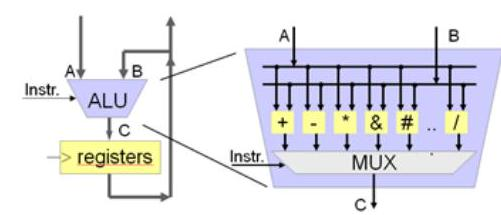
\includegraphics[width=\linewidth]{images/2025_01_02_f240dc33b50f25226887g-3(1)}
  \item registers
  \item fast but limited storage inside CPU
  \item hold intermediate results
  \item 4 / 8 / 16 / 32 / 64 bits wide
\end{itemize}

\section*{Control Unit}
\begin{itemize}
  \item Finite State Machine (FSM)
  \item reads and executes instructions\\
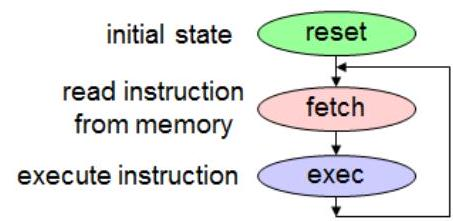
\includegraphics[width=\linewidth]{images/2025_01_02_f240dc33b50f25226887g-3}
  \item types of operations
  \item data transfer: registers $\leftarrow \rightarrow$ memory
  \item arithmetic and logic operations
  \item jumps
\end{itemize}

\section*{8. Erklären Sie den Unterschied zwischen Haupt- und Sekundärspeicher.}
Hauptstpeicher ist am Systembusangeschlossen\\
Sekundärspeicher ist über I/O angeschlossen\\
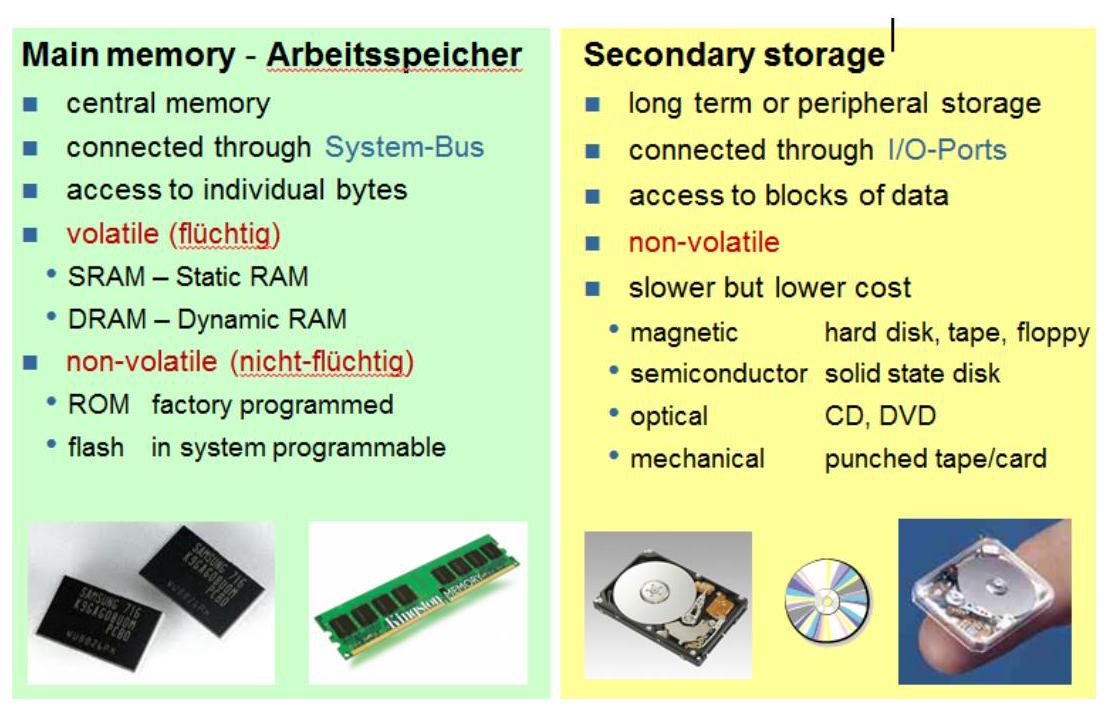
\includegraphics[width=\linewidth]{images/2025_01_02_f240dc33b50f25226887g-3(2)}\\
9. Erklären Sie den Unterschied zwischen einem PC und einem Embedded System bezüglich Aufbau, Anwendung und Programmausführung?\\
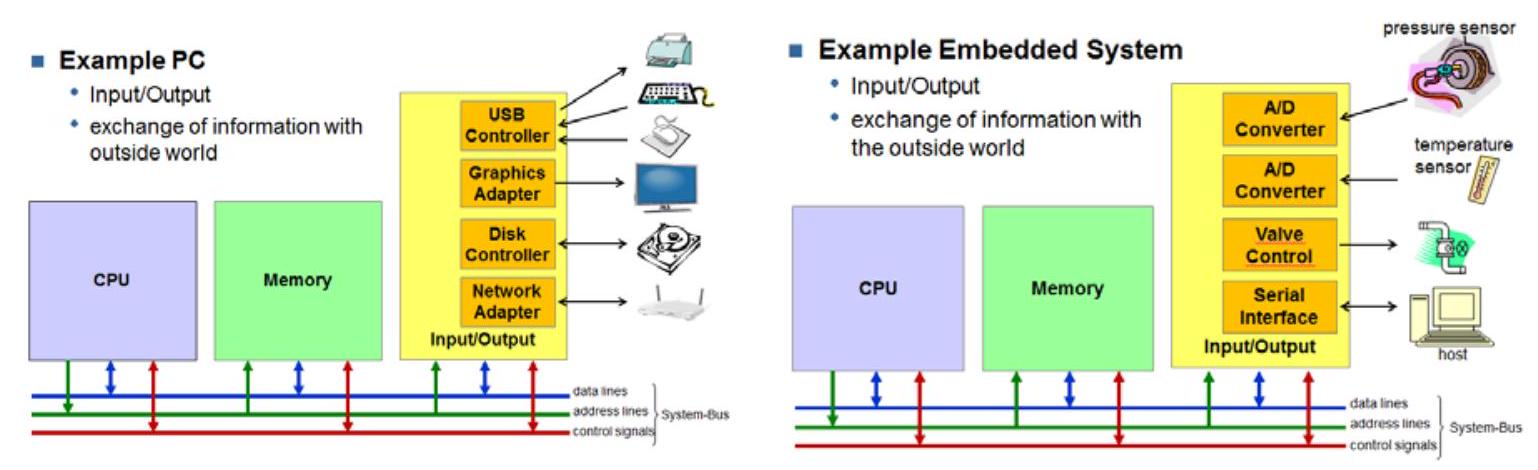
\includegraphics[width=\linewidth]{images/2025_01_02_f240dc33b50f25226887g-4}

\section*{10. Wieso ist Wissen um Assemblerprogrammierung nützlich?}
Mit Hilfe von Assembler können wir verstehen, was auf der Maschinenebene abläuft\\
Verhalten von Programmen mit Fehlern\\
Erhöhen der Performance\\
vorhandene und nicht vorhandene Optimierungen durch Compiler verstehen\\
Ursachen für ineffiziente Programme finden\\
Implementieren von System Software\\
Boot Loader, Betriebssysteme, Interrupt Service Routinen\\
Lokalisieren und vermeiden von Sicherheitslücken\\
z.B. Buffer Overflow


\end{document}